\documentclass[journal,12pt,twocolumn]{IEEEtran}

\usepackage{setspace}
\usepackage{amssymb}
\usepackage{amsthm}
\usepackage{mathrsfs}
\usepackage{longtable}
\usepackage{enumitem}
\usepackage{mathtools}
\usepackage{longtable}
\usepackage{graphicx}
\usepackage[breaklinks=true]{hyperref}

\usepackage{listings}
    \usepackage{color}                                            %%
    \usepackage{array}                                            %%
    \usepackage{longtable}                                        %%
    \usepackage{calc}                                             %%
    \usepackage{multirow}                                         %%
    \usepackage{hhline}                                           %%
    \usepackage{ifthen}                                           %%
    \usepackage{lscape}     
    \usepackage{amsmath}
       
\lstset{
%language=C,
frame=single, 
breaklines=true,
columns=fullflexible
}
\def\inputGnumericTable{}
\bibliographystyle{IEEEtran}
\newcommand{\question}{\noindent \textbf{Question: }}
\newcommand{\solution}{\noindent \textbf{Solution: }}

\title{Assignment 3}
\author{Varshini Jonnala (CS21BTECH11024)}

\begin{document}
    % make the title area
    \maketitle
    \question
    The following table gives the lifetime of $400$ neon lamps:
    \begin{table}[ht!]
            \def\ifundefined#1{\expandafter\ifx\csname#1\endcsname\relax}
\ifundefined{inputGnumericTable}
	\def\gnumericTableEnd{\end{document}}

	\documentclass[12pt%
			  %,landscape%
                    ]{report}
       \usepackage[latin1]{inputenc}
       \usepackage{fullpage}
       \usepackage{color}
       \usepackage{array}
       \usepackage{longtable}
       \usepackage{calc}
       \usepackage{multirow}
       \usepackage{hhline}
       \usepackage{ifthen}
       \usepackage[misc]{ifsym}
	\begin{document}
\else
    \def\gnumericTableEnd{}
\fi
\providecommand{\gnumericmathit}[1]{#1} 
\providecommand{\gnumericPB}[1]%
{\let\gnumericTemp=\\#1\let\\=\gnumericTemp\hspace{0pt}}
 \ifundefined{gnumericTableWidthDefined}
        \newlength{\gnumericTableWidth}
        \newlength{\gnumericTableWidthComplete}
        \newlength{\gnumericMultiRowLength}
        \global\def\gnumericTableWidthDefined{}
 \fi
 \ifthenelse{\isundefined{\languageshorthands}}{}{\languageshorthands{english}}                                                      %%
\providecommand\gnumbox{\makebox[0pt]}                       %%
\setlength{\bigstrutjot}{\jot}
\setlength{\extrarowheight}{\doublerulesep}
\setlongtables

\setlength\gnumericTableWidth{%
	50pt+%
	170pt+%
0pt}
\def\gumericNumCols{4}
\setlength\gnumericTableWidthComplete{\gnumericTableWidth+%
         \tabcolsep*\gumericNumCols*2+\arrayrulewidth*\gumericNumCols}
\ifthenelse{\lengthtest{\gnumericTableWidthComplete > \linewidth}}%
         {\def\gnumericScale{1*\ratio{\linewidth-%
                        \tabcolsep*\gumericNumCols*2-%
                        \arrayrulewidth*\gumericNumCols}%
{\gnumericTableWidth}}}%
{\def\gnumericScale{1}}


\ifthenelse{\isundefined{\gnumericColA}}{\newlength{\gnumericColA}}{}\settowidth{\gnumericColA}{\begin{tabular}{@{}p{50pt*\gnumericScale}@{}}x\end{tabular}}
\ifthenelse{\isundefined{\gnumericColB}}{\newlength{\gnumericColB}}{}\settowidth{\gnumericColB}{\begin{tabular}{@{}p{170pt*\gnumericScale}@{}}x\end{tabular}}

	\begin{center}
\begin{tabular}[c]{%
	b{\gnumericColA}%
	b{\gnumericColB}%
	}

	\hhline{|-|-~}
	 \multicolumn{1}{|p{\gnumericColA}|}%
	{\gnumericPB{\centering}\gnumbox{\textbf{Event}}}
	&\multicolumn{1}{p{\gnumericColB}|}%
	{\gnumericPB{\centering}\gnumbox{\textbf{Description}}}
\\
    \hhline{|--|~}
	 \multicolumn{1}{|p{\gnumericColA}|}%
	{\gnumericPB{\centering}\gnumbox{$X=0$}}
	&\multicolumn{1}{p{\gnumericColB}|}%
	{\gnumericPB{\centering}\gnumbox{Hanif losing the game}}
\\
    \hhline{|--|~}
	 \multicolumn{1}{|p{\gnumericColA}|}%
	{\gnumericPB{\centering}\gnumbox{$X=1$}}
	&\multicolumn{1}{p{\gnumericColB}|}%
	{\gnumericPB{\centering}\gnumbox{Hanif winning the game}}
\\
\hhline{|-|-|~}
\end{tabular}
	\end{center}
	
\ifthenelse{\isundefined{\languageshorthands}}{}{\languageshorthands{\languagename}}
\gnumericTableEnd

        \caption{Given Data}
	        \label{Tables:Table}
    \end{table}
    \begin{enumerate}[label=(\roman*)]
		\item Represent the given information with the help of a histogram.
		\item How many lamps have a lifetime of more than $700$ hours?
    \end{enumerate}
    \solution 
     \begin{enumerate}[label=(\roman*)]
         \item Representation of given information in the form of histogram:
         \begin{figure}[!ht]
		    \centering
		    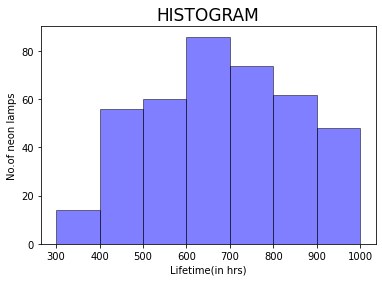
\includegraphics[width=\columnwidth]{prv3.png}
		    \caption{Histogram}
        \label{fig:fig-1}
    	\end{figure}
	
         \item Clearly, from the given table, The number of lamps that have a lifetime of more than $700$ hours would be 
         \begin{align}
              &= 74 + 62 + 48 \\
              &= 184
         \end{align}
     \end{enumerate}
\end{document} 
